\documentclass[11pt]{article}
%Gummi|065|=)

\title{\textbf{High Performance Computing Exercises}}
\author{Calum Pennington}
\date{} % Remove date

\usepackage[margin=1.5cm]{geometry} % Set page margins
\usepackage{graphicx}
\usepackage{caption}
\usepackage{subcaption}

\usepackage[T1]{fontenc}
\usepackage{helvet}
\renewcommand{\familydefault}{\sfdefault}
% Set font

\usepackage{csvsimple}
\usepackage{pdflscape, adjustbox}

\begin{document}
\maketitle

\section*{Neutral Theory Simulations}
% '*' - remove section numbers

\subsection*{Question 7}

\begin{figure}[h]
\centering
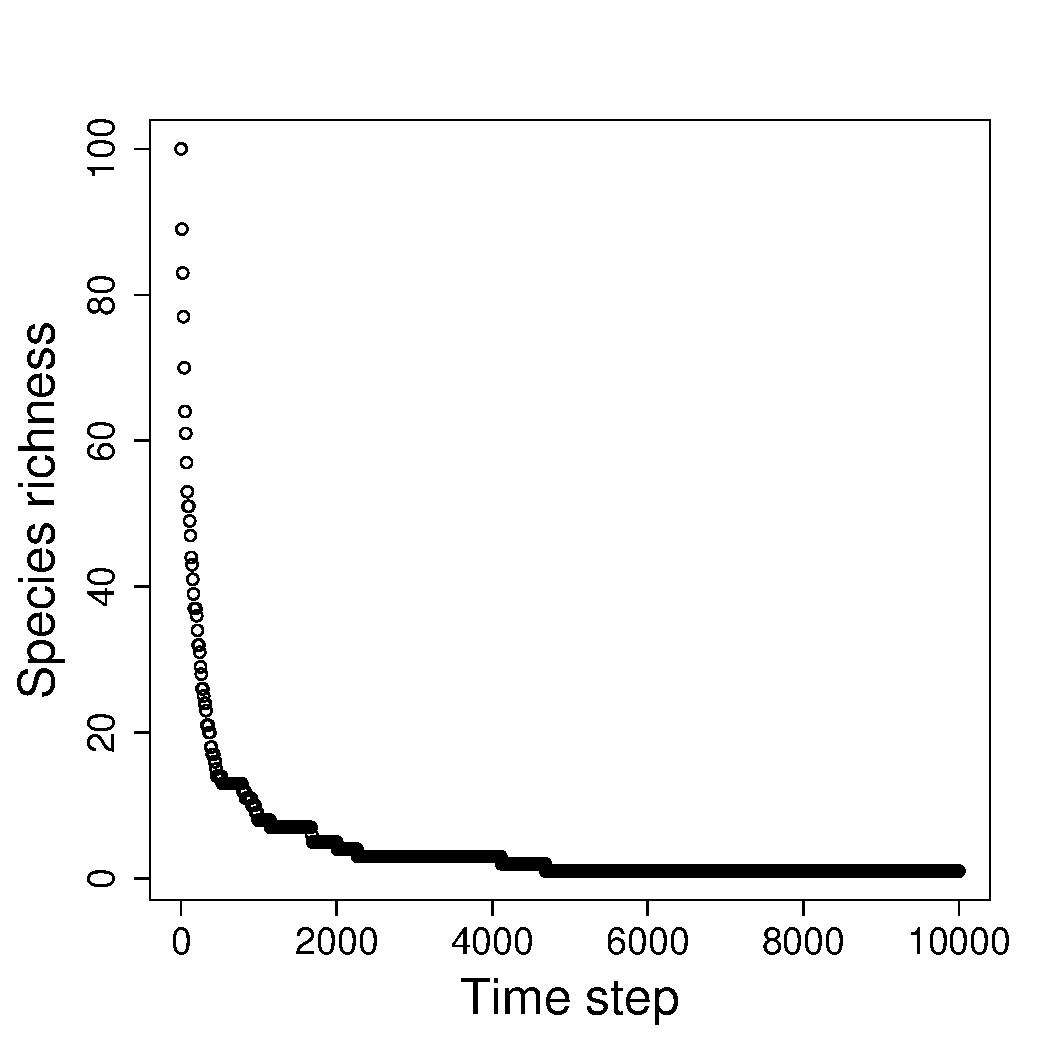
\includegraphics[width=0.5\linewidth]{../Results/Question_7.pdf}
\caption{A time series of species richness during a neutral model simulation (initial state of max diversity; system size 100 individuals; no speciation).}
\end{figure}

Classic Neutral Theory, models a community of J individuals. At every time step, a randomly-chosen individual dies and is replaced by an offspring of another randomly-chosen individual. Given long enough, the system always converges to a single-species state. Without speciation to replenish species, gradual extinctions due to drift guarantee that only a one species remains.

\newpage

\subsection*{Question 10}
\begin{figure}[h]
\centering
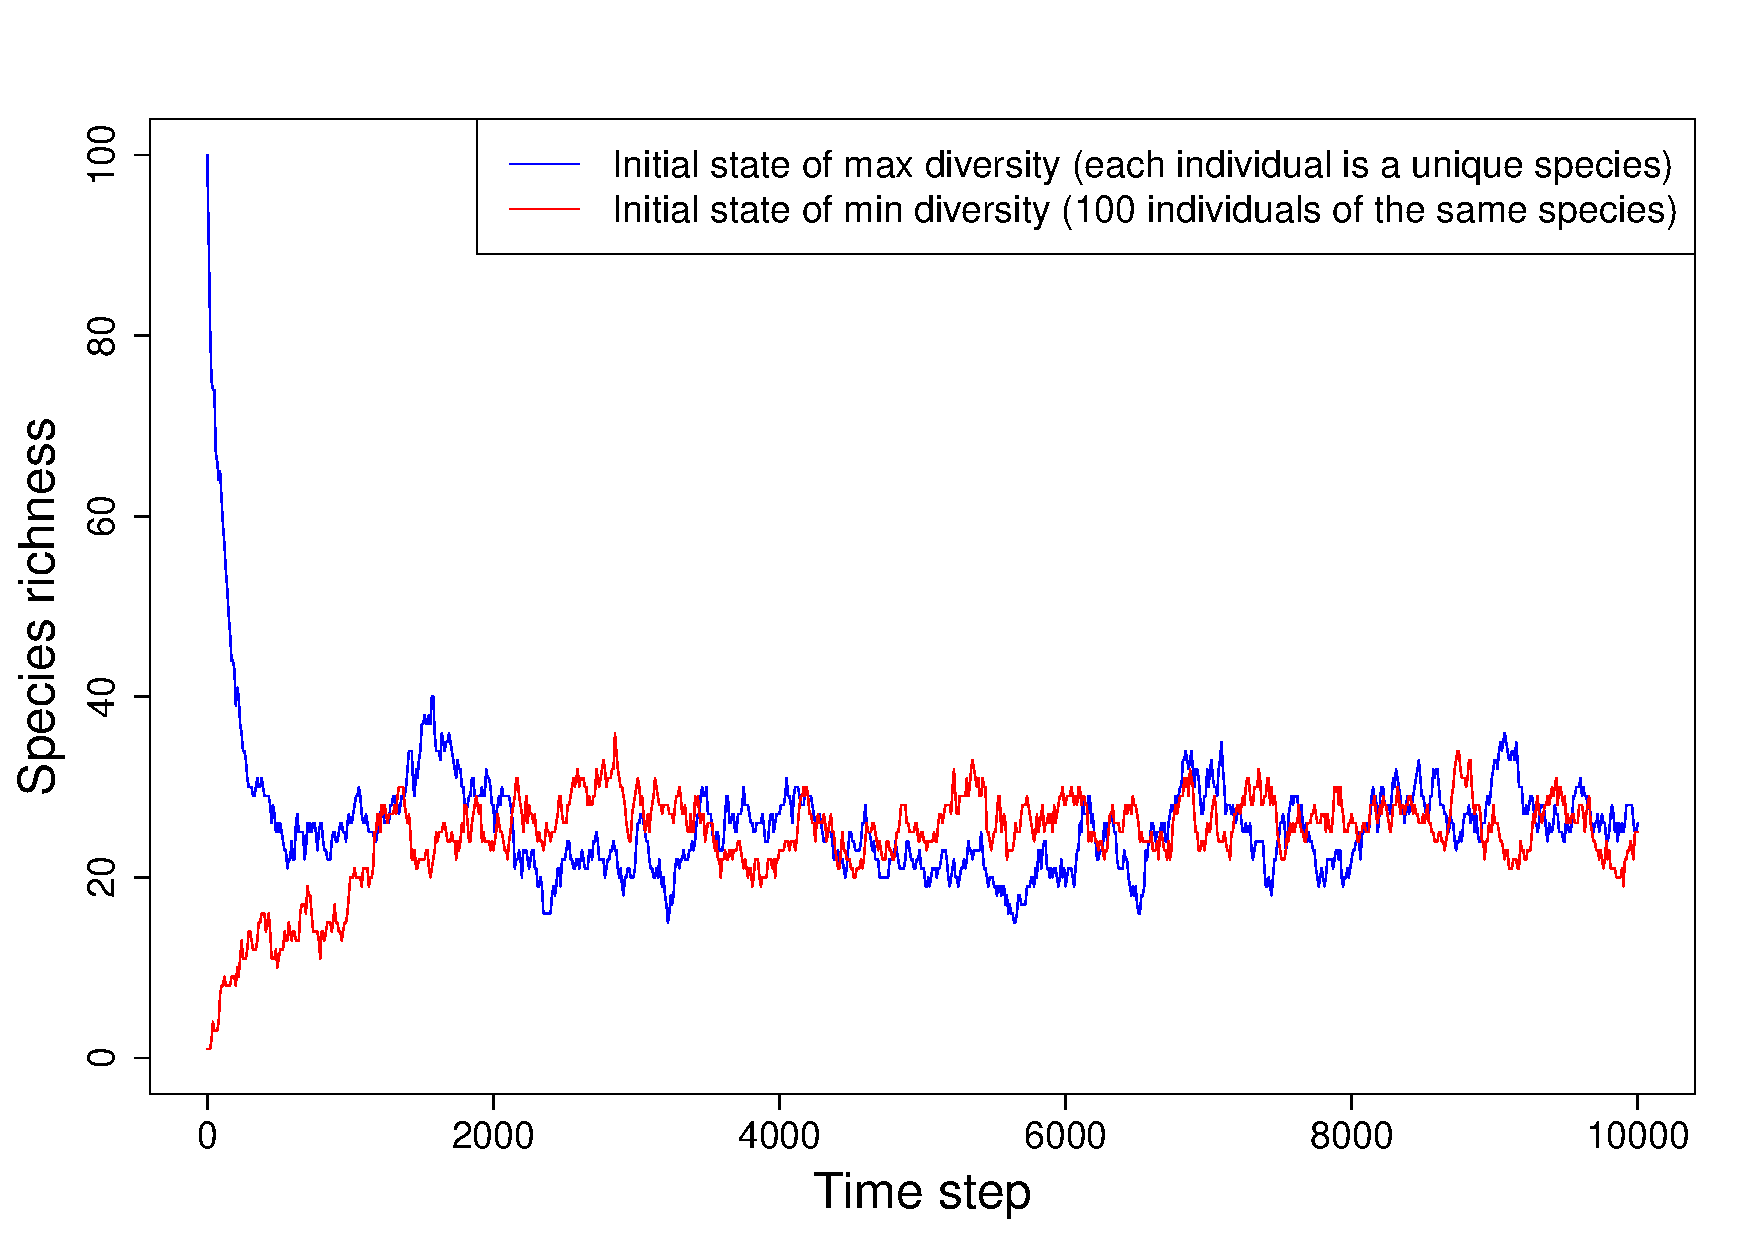
\includegraphics[width=0.8\linewidth]{../Results/Question_10.pdf}
\caption{Time series of species richness for two neutral model simulations, with different initial states (system size 100 individuals; speciation rate 0.1).}
\end{figure}

'Initial state' refers to the simulation community's species richness at time 0. Neutral models simulate death and speciation, so species richness inevitably changes. (A species goes extinct if it has an abundance of one individual, and that individual dies.) A system is in dynamic equilibrium when its species richness is relatively constant (but fluctuates) (very small systems are an exception).

Given long enough, systems (of equal size, with the same speciation rate) converge to similar species richness, regardless of their initial state. Species richness at equilibrium is determined, not by the initial state, but a balance between extinction (due to drift) and speciation.

Birth and death (thus extinction and species abundances) are stochastic: every individual has an equal chance of being chosen (either to die or reproduce). Speciation is random too, but it occurs with a probability, v, that we can set. So, specifically, speciation rate sets the system's diversity at equilibrium. The higher the speciation rate, the higher the richness. A speciation rate of one (dead individuals are always replaced by new species) guarantees max diversity at equilibrium. Without speciation, simulations result in monodominance.

\newpage

\subsection*{Question 14}
\begin{figure}[h]
\centering
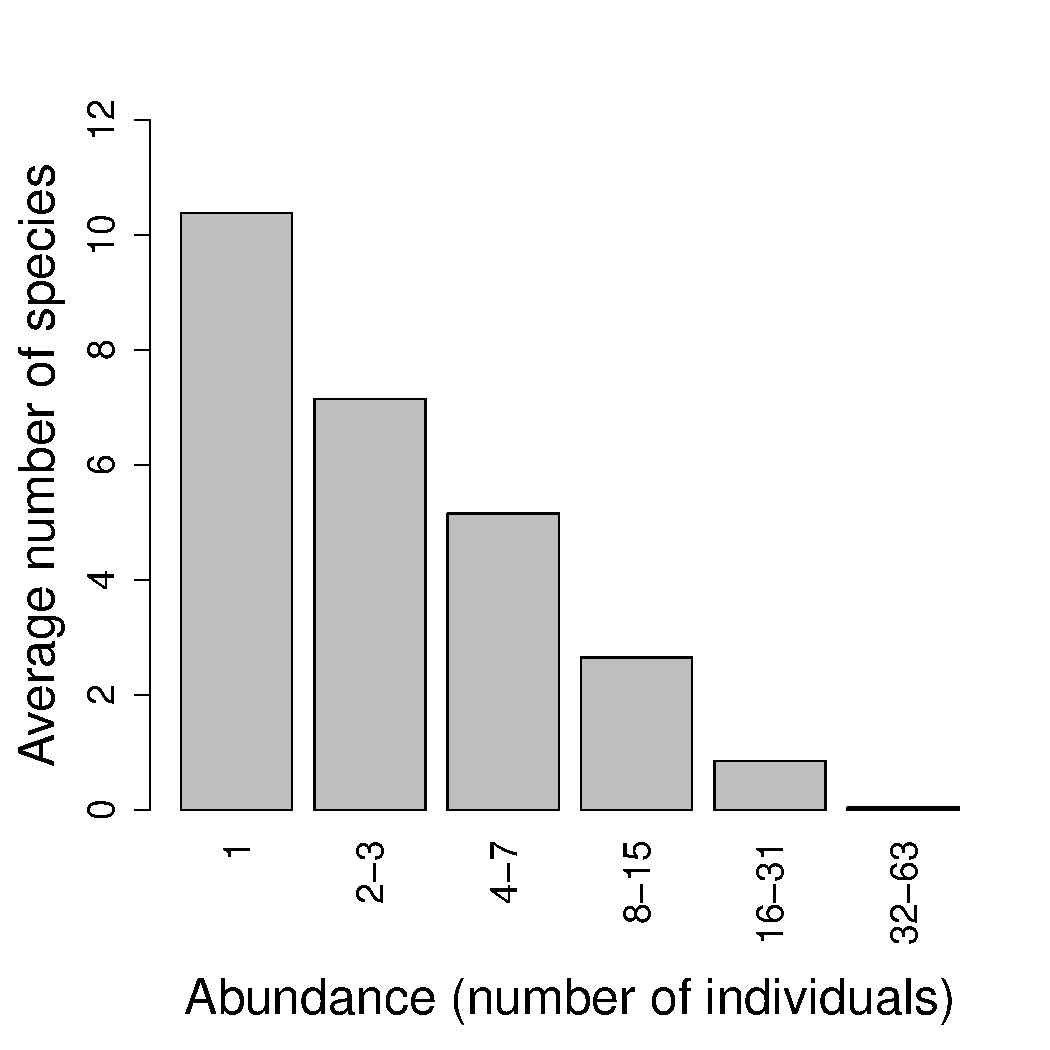
\includegraphics[width=0.5\linewidth]{../Results/Question_14.pdf}
\caption{\emph{Mean Species Abundance Distribution (as Octaves)}\\\\
At intervals during a neutral model simulation (system size 100 individuals; speciation rate 0.1), we recorded the system's species abundance distribution. We took readings after a 'burn in' period, when the system had settled. We sorted abundances into 'octave classes', e.g. how many species had an abundance of 2 or 3 individuals.}
\end{figure}

\newpage

%\begin{landscape}
\subsection*{Question 17}
\begin{figure}[h]
\centering
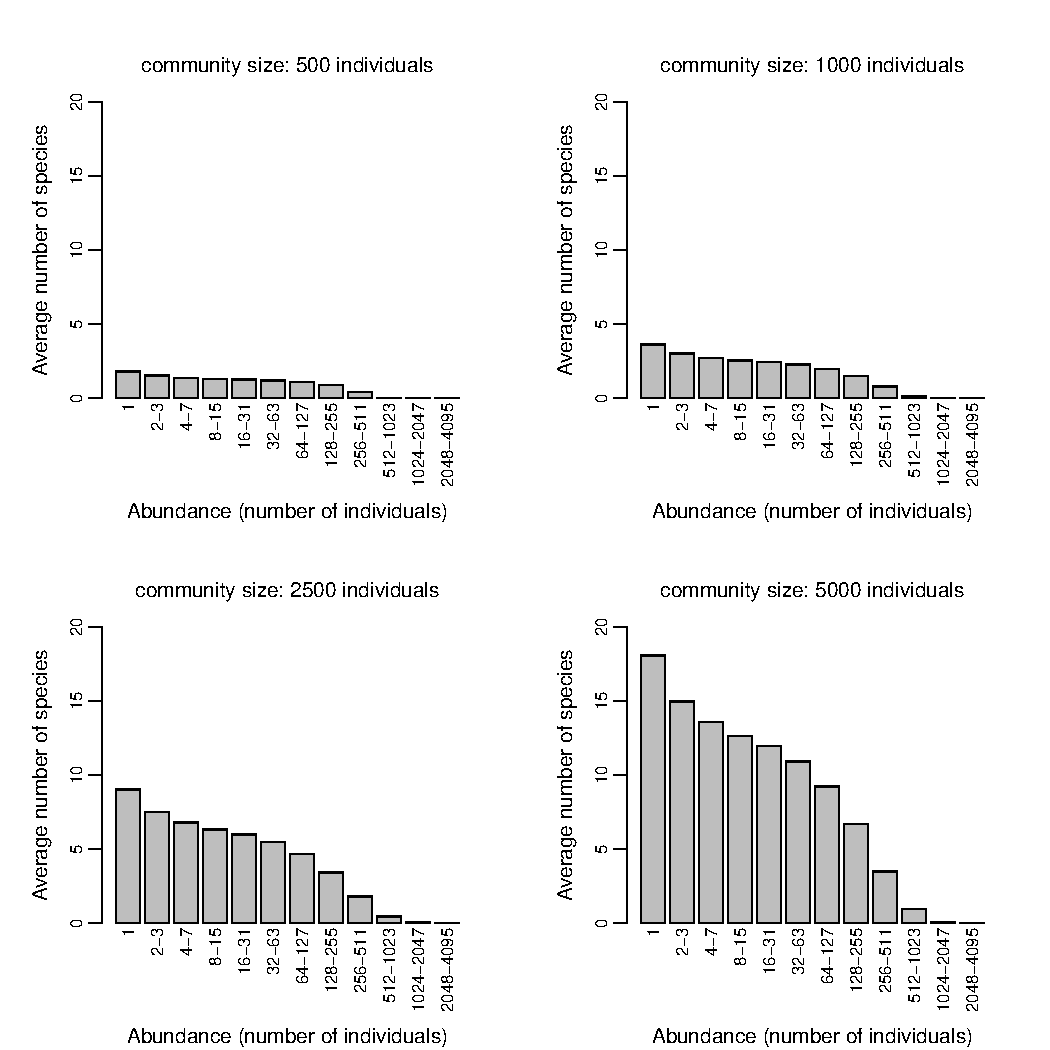
\includegraphics[width=0.8\linewidth]{../Results/Question_17.pdf}
\caption{\emph{Mean Species Abundance Distribution (as Octaves)}\\\\
We ran twenty-five neutral model simulations per community size (speciation rate 0.003617). At intervals during a simulation, we recorded the system's species abundance distribution. The mean excludes data from a 'burn in' period, before the system had settled. We sorted abundances into 'octave classes', e.g. how many species had an abundance of 2 or 3 individuals.}
\end{figure}

%\begin{landscape}

\begin{table}[]
\centering
%\resizebox{\textwidth}{!}{%
\begin{tabular}{lllll}
\multicolumn{1}{c}{\textbf{Abundance octaves}} & \multicolumn{4}{c}{\textbf{Community size}} \\
 & \textit{500} & \textit{1000} & \textit{2500} & \textit{5000} \\
\textit{1} & 1.80910705 & 3.616458885 & 9.023969911 & 18.068619782 \\
\textit{2-3} & 1.504177791 & 3.000266728 & 7.514763669 & 14.958472588 \\
\textit{4-7} & 1.365026155 & 2.715393113 & 6.783181767 & 13.579961601 \\
\textit{8-15} & 1.291080868 & 2.553138136 & 6.33334456 & 12.627035483 \\
\textit{16-31} & 1.237014211 & 2.421672719 & 5.981778377 & 11.953921638 \\
\textit{32-63} & 1.174635878 & 2.250649931 & 5.479925901 & 10.898243618 \\
\textit{64-127} & 1.06968365 & 1.965689453 & 4.673054901 & 9.235084975 \\
\textit{128-255} & 0.866693836 & 1.485151399 & 3.421612215 & 6.678944749 \\
\textit{256-511} & 0.41384392 & 0.775758793 & 1.792949366 & 3.492000284 \\
\textit{512-1023} & 0 & 0.123605709 & 0.455226227 & 0.950721752 \\
\textit{1024-2047} & 0 & 0 & 0.018794207 & 0.068619782 \\
\textit{2048-4095} & 0 & 0 & 0.000011227 & 0.000071109
\end{tabular}%
%}
\caption{Mean Species Abundance Distribution (as Octaves) (per community size, the mean number of species in each octave class)}
\label{my-label}
\end{table}

%\end{landscape}

\clearpage

\subsection*{Challenge C}
\begin{figure}[h]
\centering
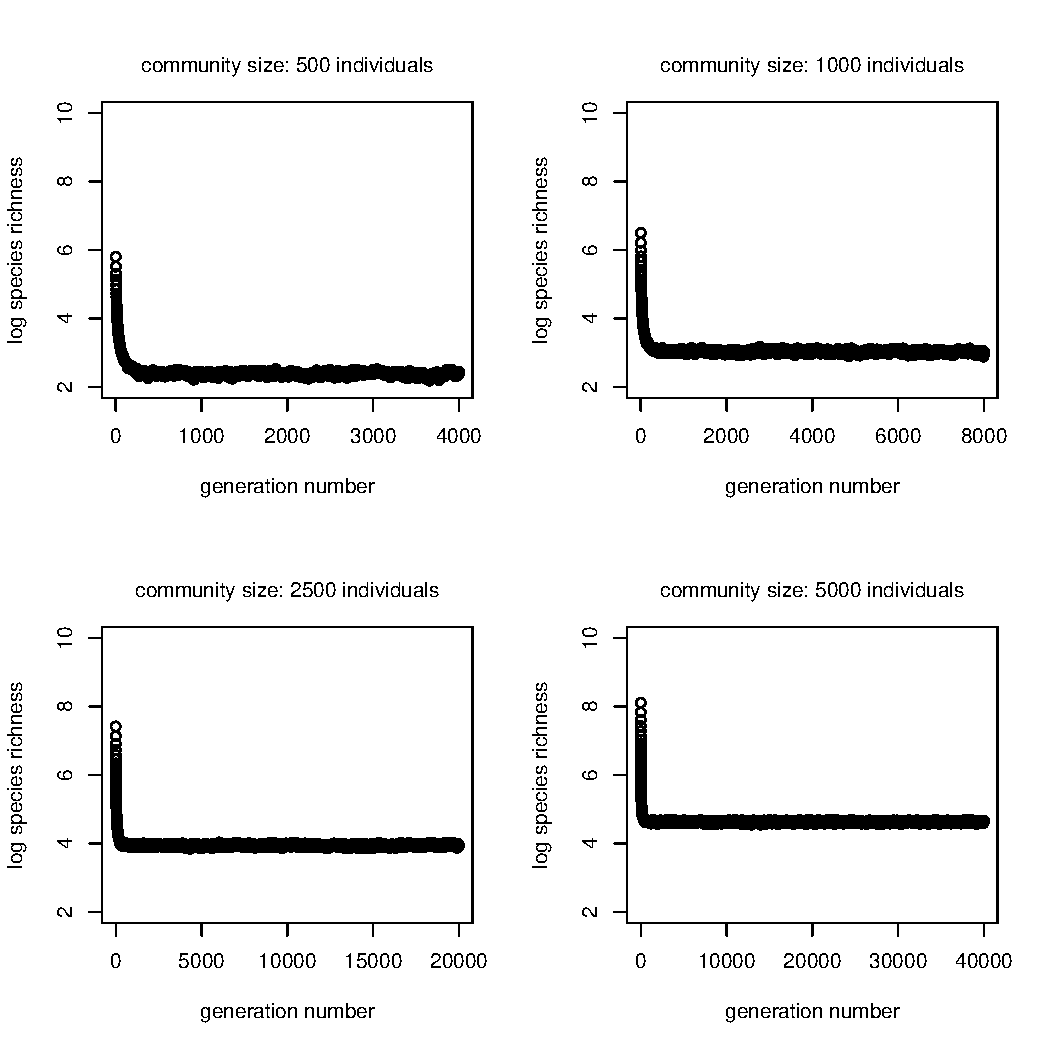
\includegraphics[width=0.8\linewidth]{../Results/Challenge_C.pdf}
\caption{\emph{Time Series of Mean Species Richness during the Burn In}\\\\
We ran twenty-five neutral model simulations per community size (speciation rate 0.003617). Per simulation, we recorded species richness at intervals during a 'burn in' period (before the system had settled).
at every step of . The burn in lasted size * 8 steps.}
\end{figure}

\newpage

% **Too small?
\subsection*{Challenge A}
\begin{figure}[h]
\centering
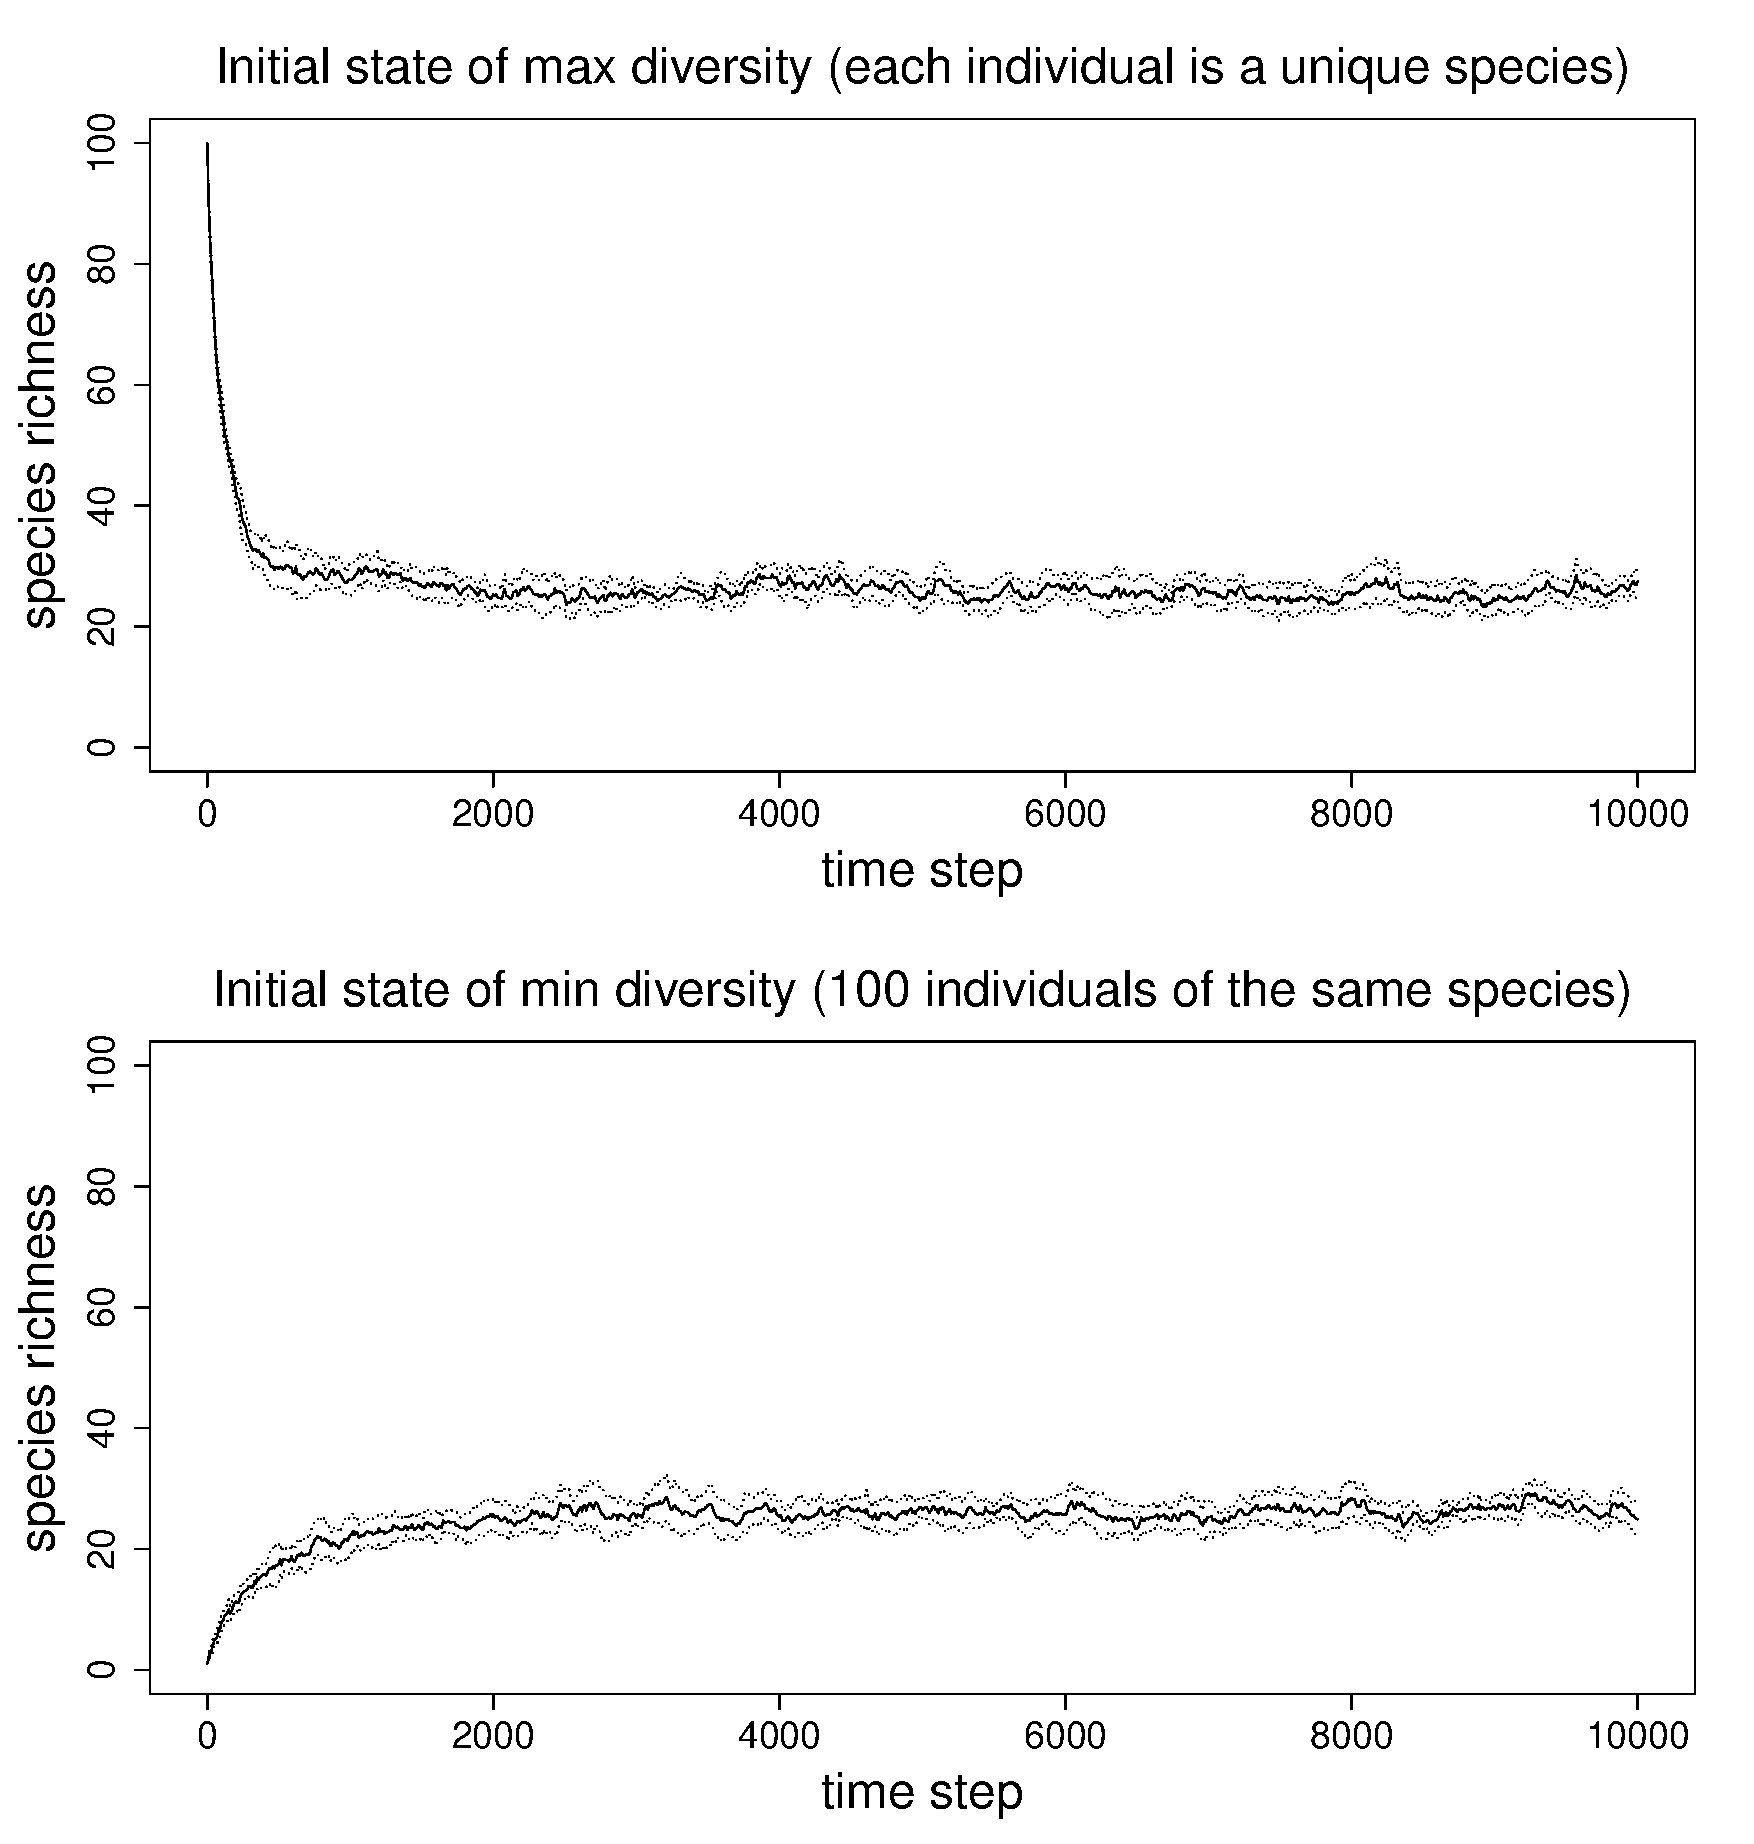
\includegraphics[width=0.8\linewidth]{../Results/Challenge_A.pdf}
\caption{Time series of mean species richness for neutral model simulations, with different initial states (system size 100 individuals; speciation rate 0.1). Dotted lines show 97.2\% confidence intervals. We recorded species richness at intervals during a simulation and ran ten simulations per initial state.} % **Specify intervals?
% We ran ten simulations per initial state. Per simulation, we recorded species richness at intervals.
\end{figure}

For a system size of 100 individuals and speciation rate 0.1, it takes approximately 2000 time steps to reach equilibrium. This is slow, so the total size of the simulation will be limited by computer memory.

\newpage

\subsection*{Challenge B}
\begin{figure}[h]
\centering
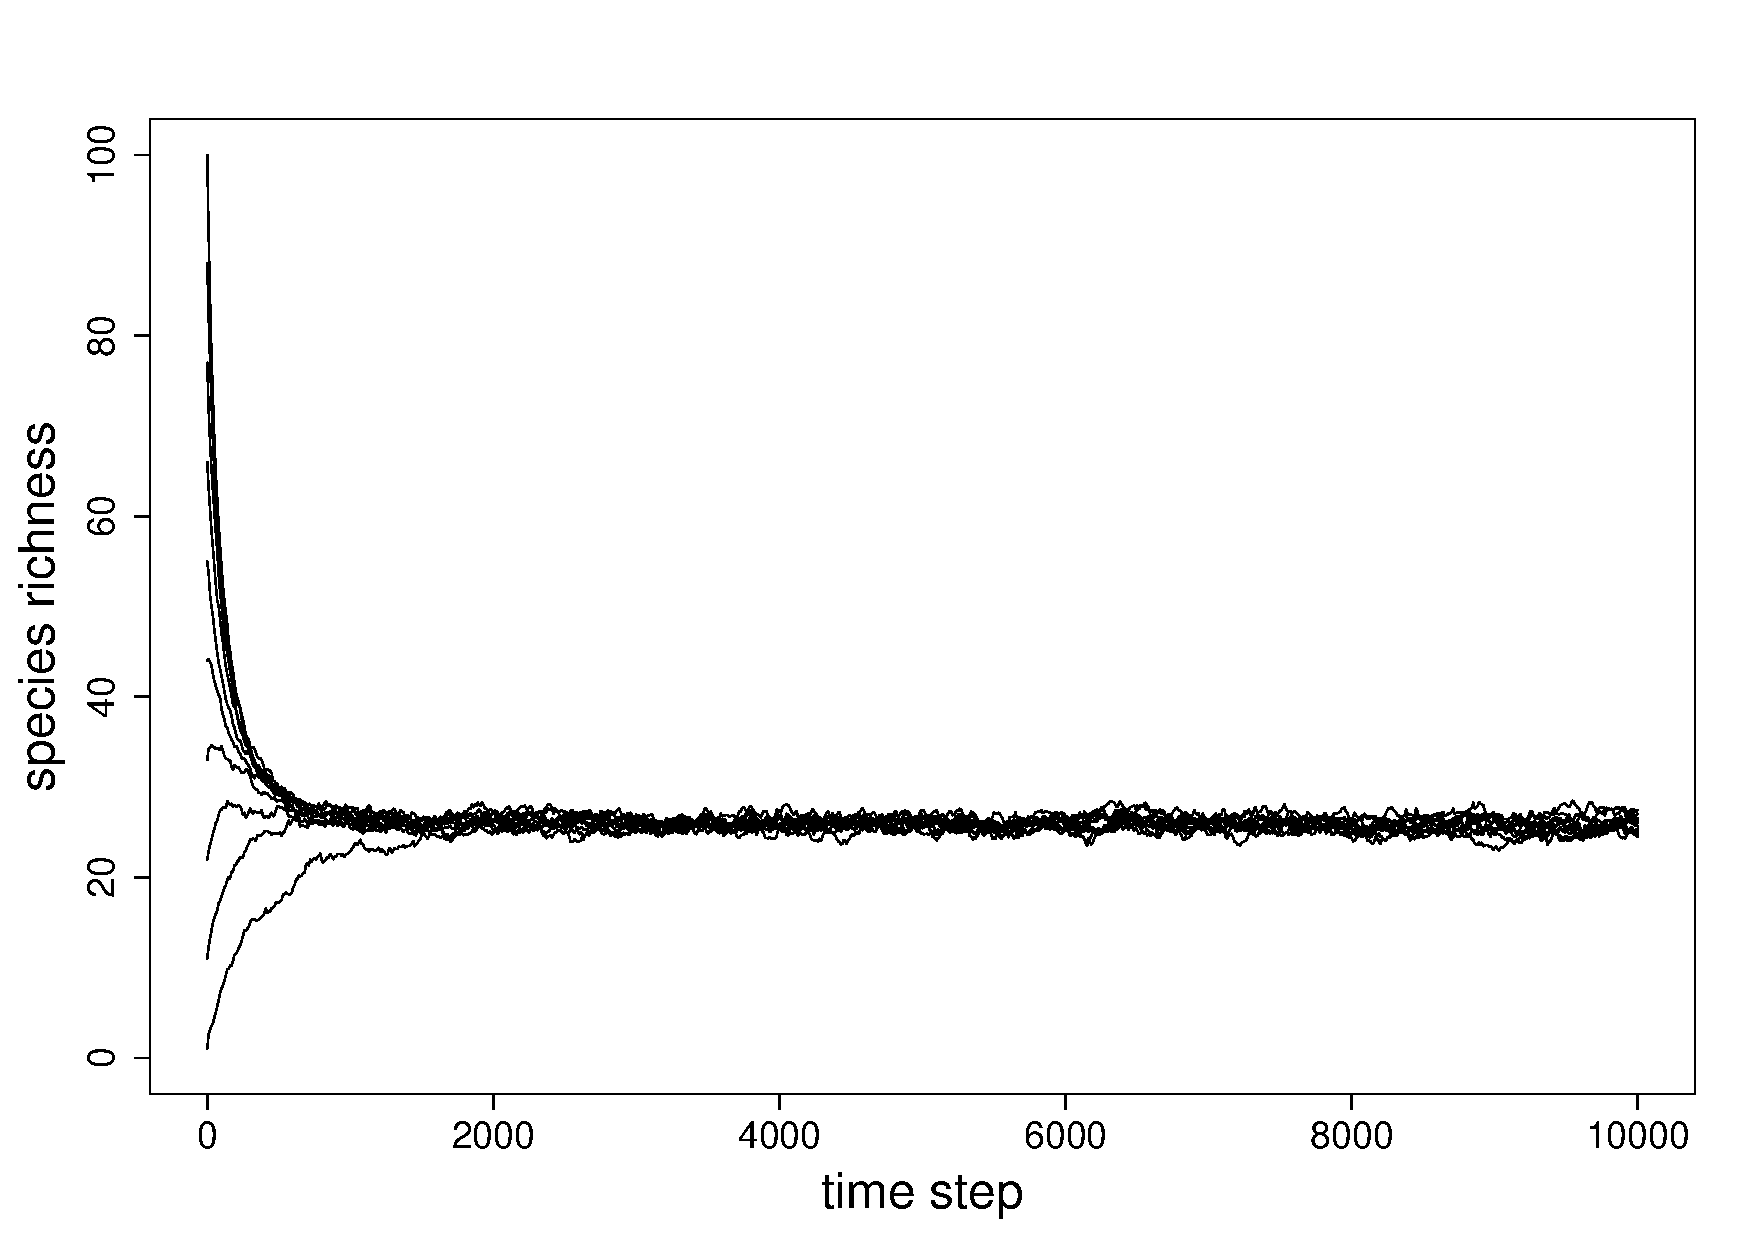
\includegraphics[width=0.8\linewidth]{../Results/Challenge_B.pdf}
\caption{\emph{Time Series of Mean Species Richness for Neutral Model Simulations, with Different Initial States}\\\\
'Initial state' refers to the simulation community's species richness at time 0. We ran twenty-five simulations (system size 100 individuals; speciation rate 0.1) for each of ten different initial states. Per simulation, we recorded species richness every ten steps.}
\end{figure}

\subsection*{Challenge D}

We ran one hundred simulations on a high performance computing cluster, one simulation per node. Each simulation ran for 11.5 hours (though we ran them in parallel), so we used 1150 (11.5 * 10) CPU hours. In contrast, using coalescence, I ran the same simulations on my own computer in under 30 seconds. Coalescence is much faster.

Without coalescence, we start with an initial state and, applying the rules of the model, take the system forward until equilibrium. This is slow (it can take many steps) and simulation size is limited by computer memory. Coalescence is more efficient. It begins with a present-day state and works backwards in time, applying the rules in reverse. You do not wait for the system to equilibrate.

\newpage

\section*{Fractals}

\subsection*{18)}
Doubling the lengths of a polygon's edges, multiplies its area by four. This is two (ratio of the new to old length) to the power of two (the polygon's dimension). But, if we double the lengths of a fractal, its spatial content scales by a power that is not an integer.

\noindent
\\
A fractal can be split into parts, each of which is (at least approximately) a smaller copy of the whole.

\noindent
\\
A fractal's size (number of parts) = width of a part to the power of the fractal's dimension.

\subsubsection*{Sierpinski carpet}
size = width$^{x}$\\
log(size) = xlog(width)\\
log(size) \textbackslash\ log(width) = x\\
log(8) \textbackslash\ log(3) = 1.89 (2 d. p.)

\subsubsection*{Menger sponge}
log(20) \textbackslash\ log(3) = 2.73 (2 d. p.)

\newpage

\subsection*{19) Chaos Game}
\begin{figure}[h]
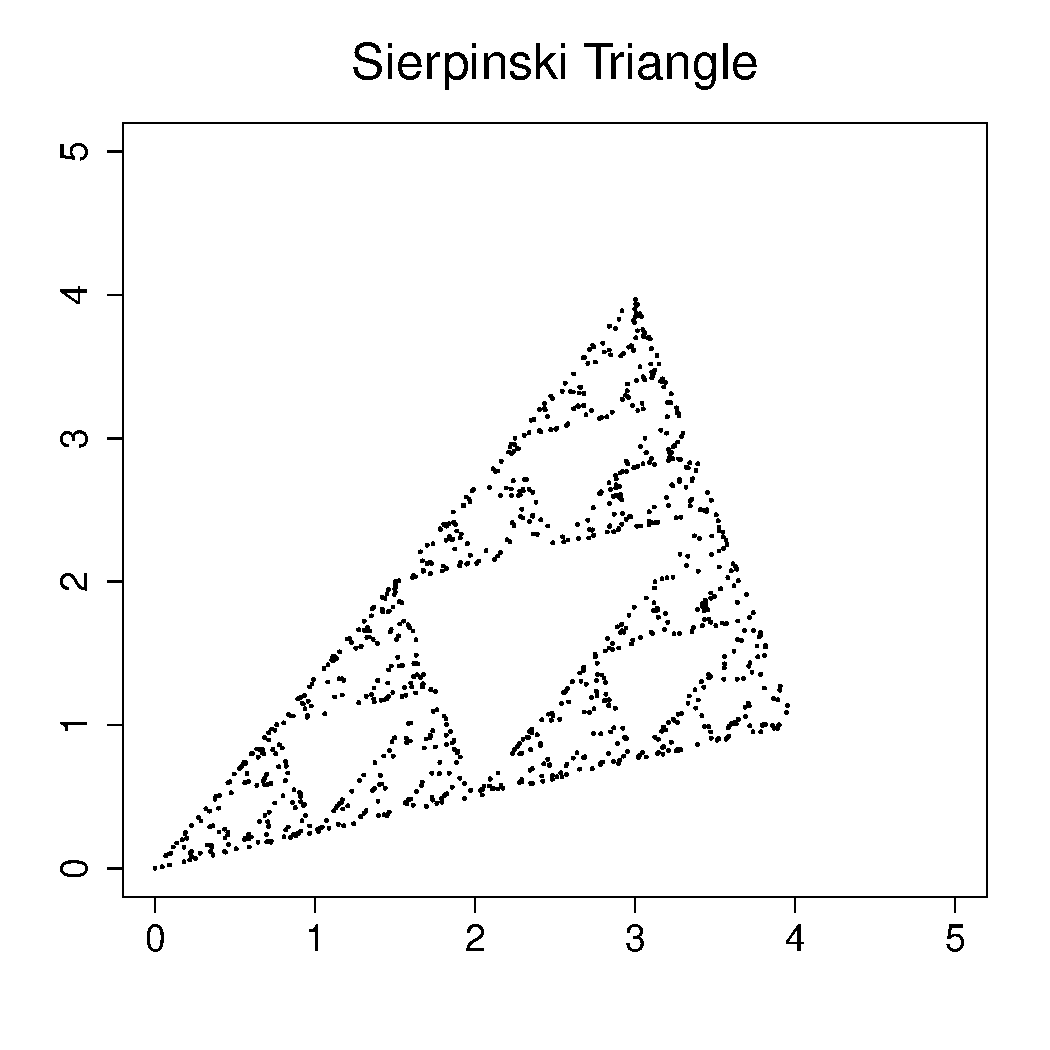
\includegraphics[width=0.5\linewidth]{../Results/19_chaos_game.pdf}
%\caption{}
\end{figure}

Regardless of the initial position (X), 'chaos\_game' draws the same shape (providing A, B, C and the distance of movement towards the next point are constant). Each iteration of 'chaos\_game' moves X closer to A, B or C and plots a point at X. So, A, B and C set the shape's edges by restricting where the function can plot points. If X is far away from A, B and C, each iteration brings it closer and eventually bounds it within them. Once inside the vertices, X can not leave. Thus, change A, B or C, not X, to draw a differently-shaped triangle.

\subsection*{Challenge E}
\begin{figure}[h]
5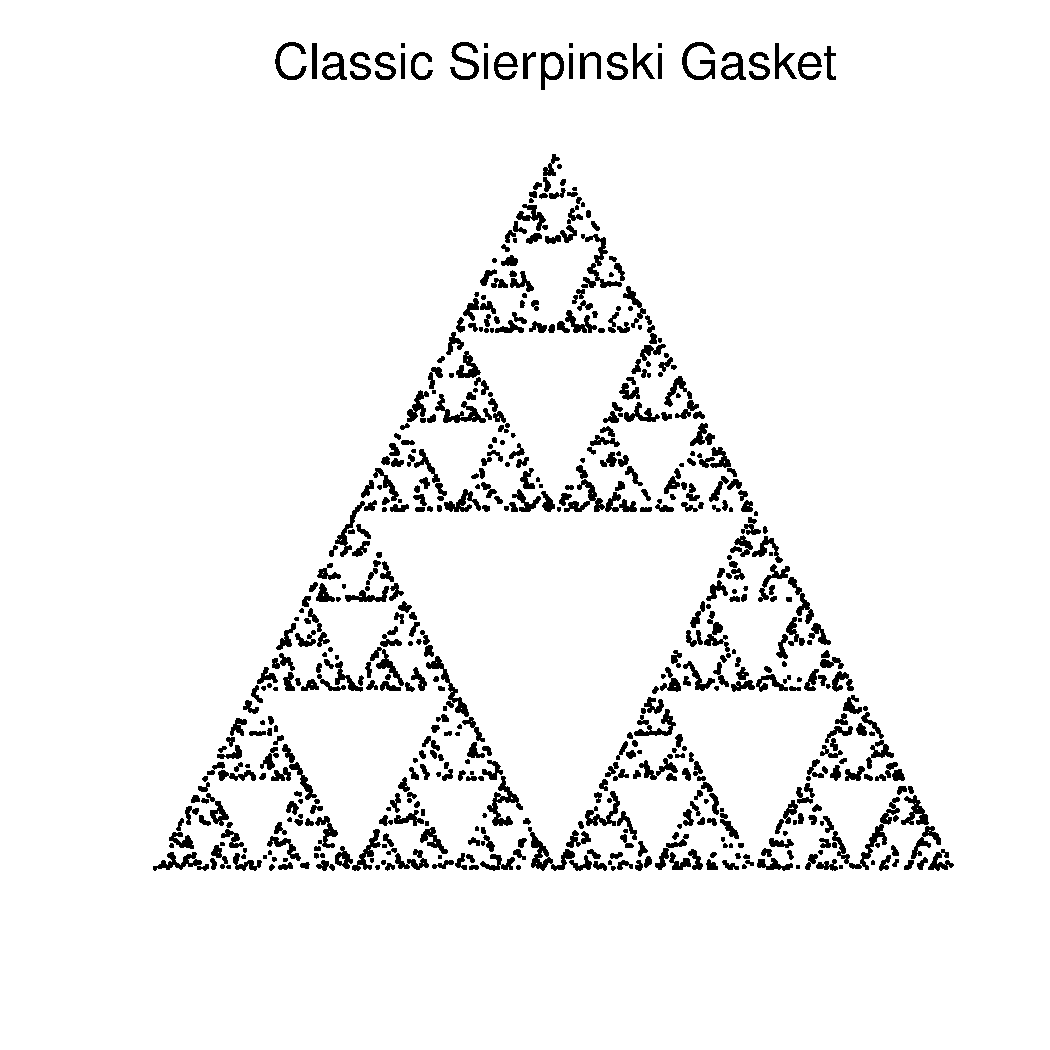
\includegraphics[width=0.5\linewidth]{../Results/19_Classic_Sierpinski_Gasket}
\end{figure}

\newpage

\subsection*{22) Spiral}
\begin{figure}[h]
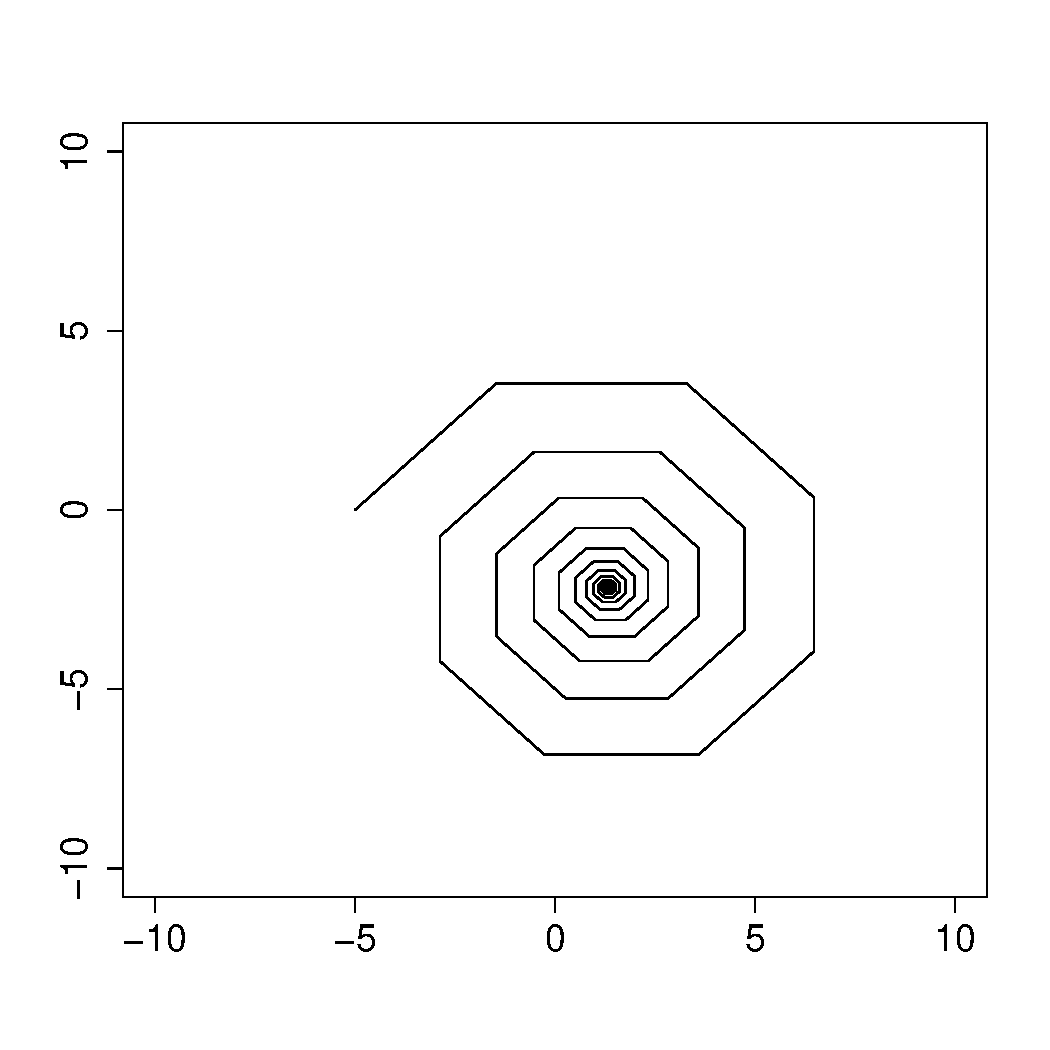
\includegraphics[width=0.5\linewidth]{../Results/22_spiral.pdf}
\end{figure}

The basic function of 'spiral' is to draw a line using 'turtle'. The function repeatedly calls itself, so draws lots of lines. There is no condition to stop the calls, so it is an infinite loop. To manage the size of its workspace (memory available for data storage), R limits the number of nested expressions that will be evaluated. An error is thrown once the limit is reached.

\subsection*{23) spiral\_2}
\begin{figure}[h]
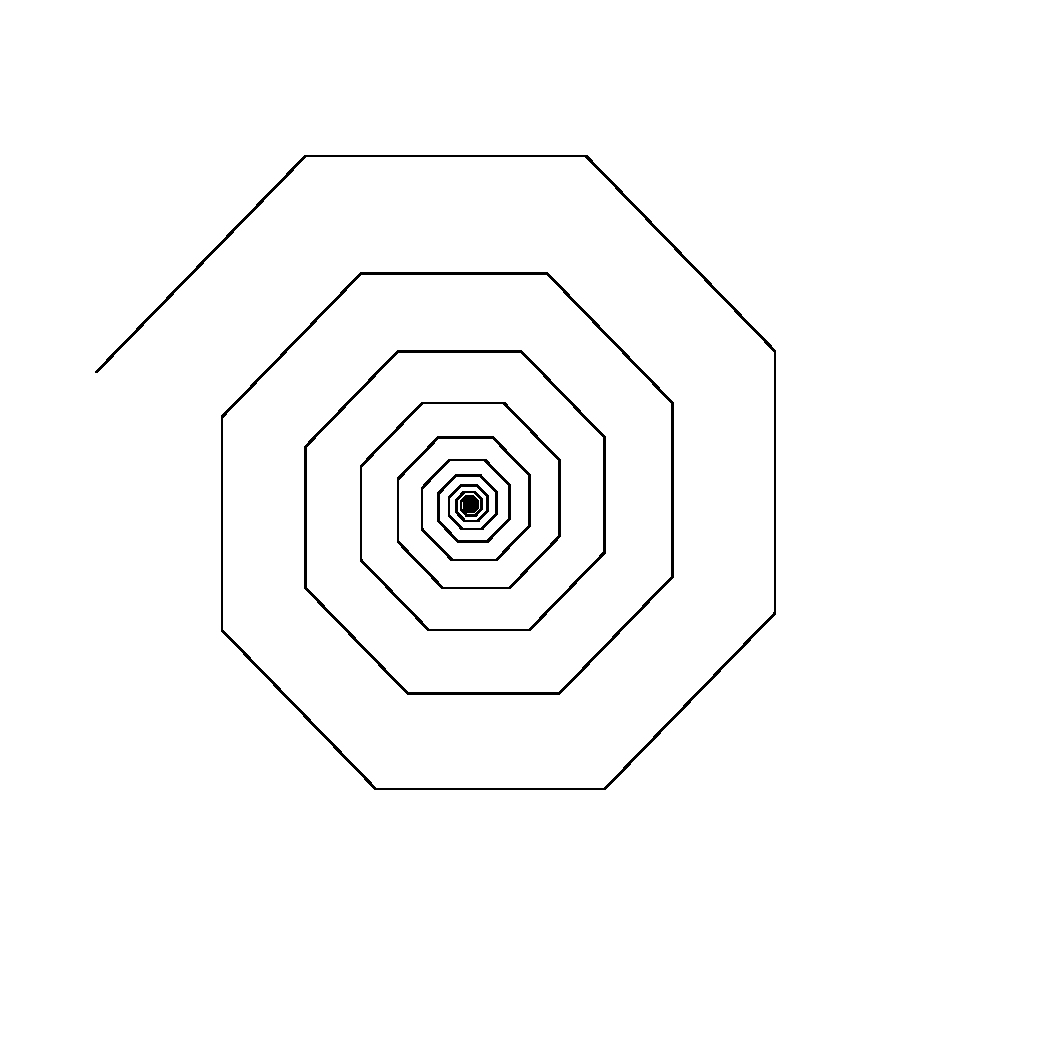
\includegraphics[width=0.5\linewidth]{../Results/23_spiral_2.pdf}
\end{figure}

\newpage

\subsection*{24) Tree}
\begin{figure}[h]
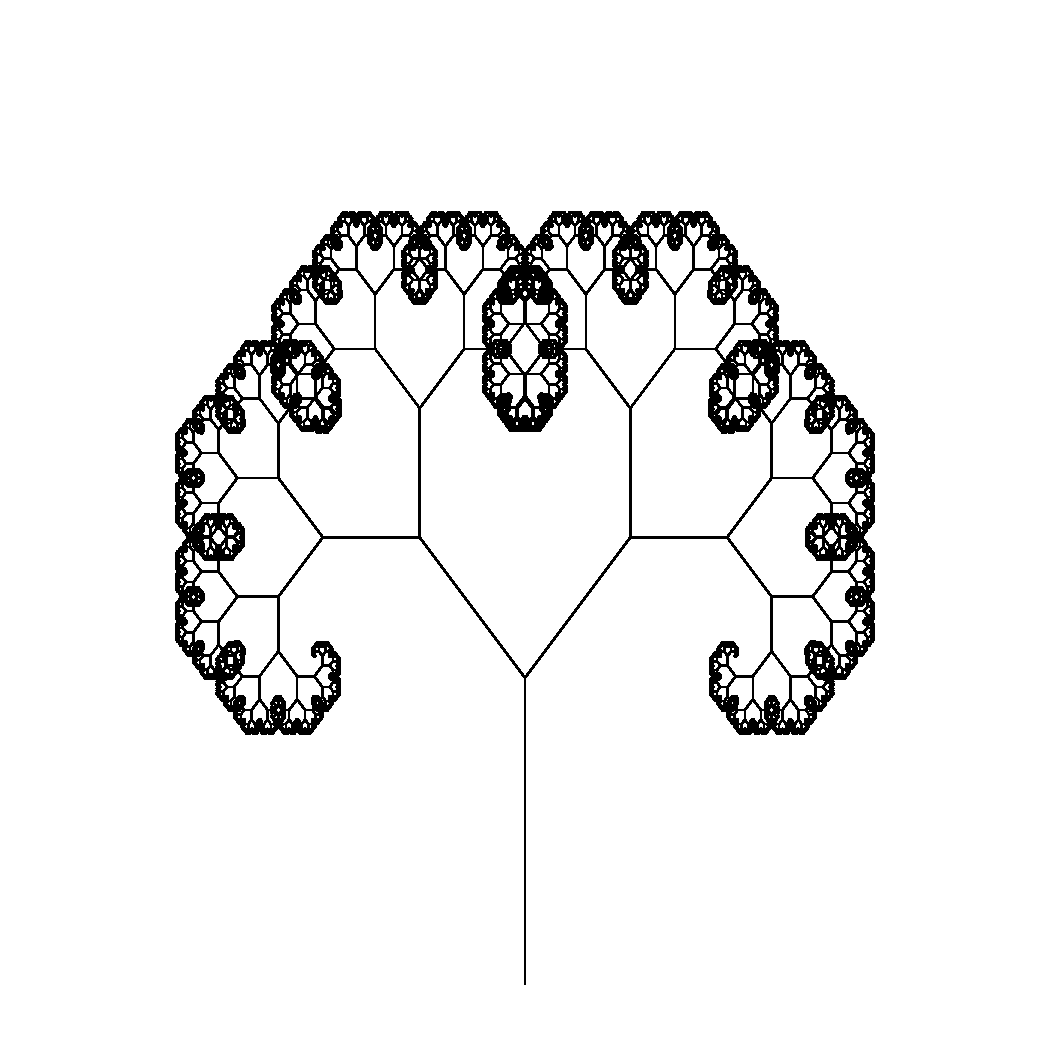
\includegraphics[width=0.5\linewidth]{../Results/24_tree.pdf}
\end{figure}

\newpage

\subsection*{26) fern\_2}
\begin{figure}[h]

\includegraphics[width=0.8\linewidth]{../Results/26_fern_2.pdf}
\end{figure}

\subsection*{Challenge F}
\begin{figure}[h]
%\includegraphics[width=0.8\linewidth]{../Results/Challenge_F.pdf}
\end{figure}

The basic function of 'fern\_2' is to draw a line using 'turtle'. The function repeatedly calls itself, so draws lots of lines. Each time, it uses new argument values, so the next line is a different direction and length. The function is recursive - it continually calls itself until you stop the process. Here, it stops if 'length' falls below a threshold 'e'. If e is high, the function draws fewer lines: there may be so few, the image does not resemble a fern. The lower e's value, the longer the function is stuck in recursion. The function draws a more detailed fern, but uses more computer memory and is slower.

\newpage

\subsubsection*{Experimenting with the variables of fern and tree}
\begin{figure}[h]
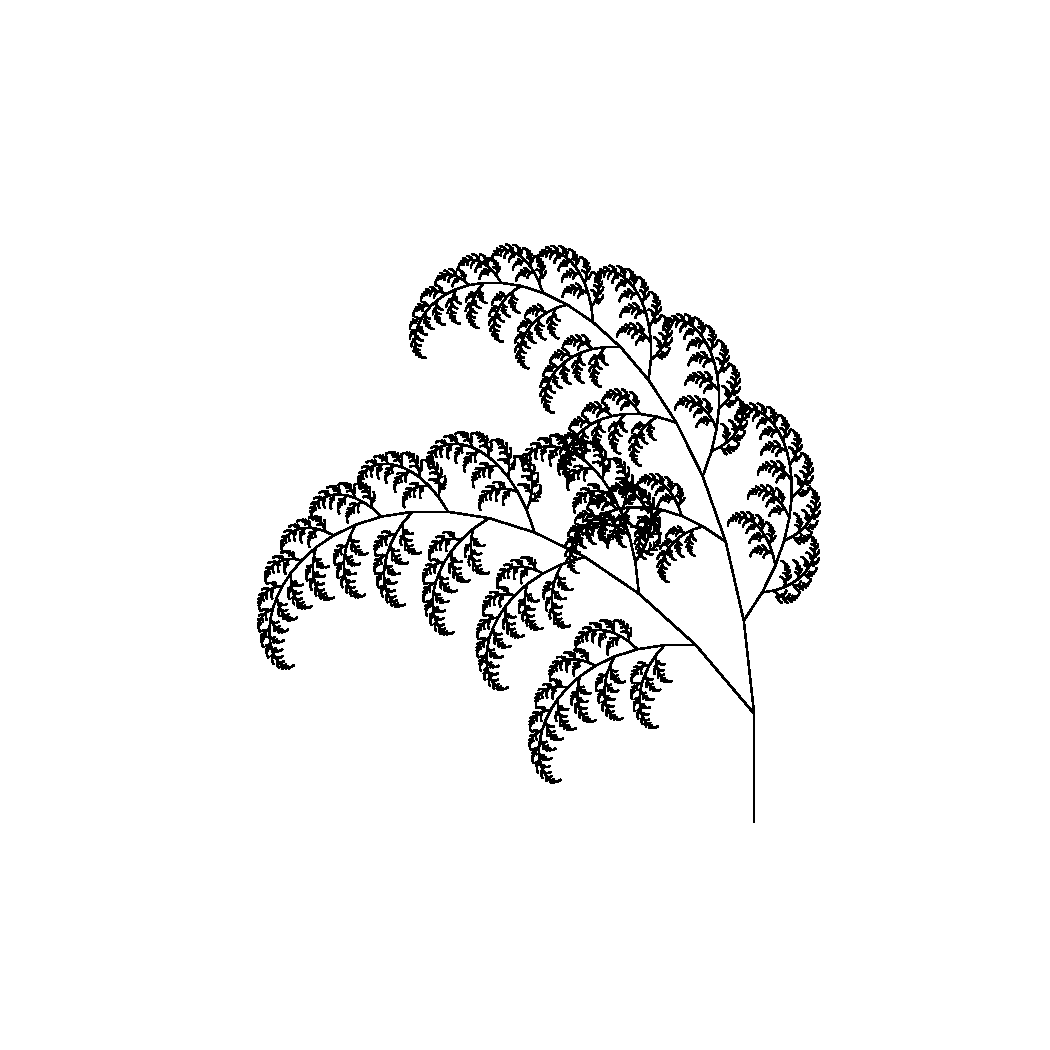
\includegraphics[width=0.5\linewidth]{../Results/Challenge_F_Fern.pdf}
\end{figure}

\begin{figure}[h]
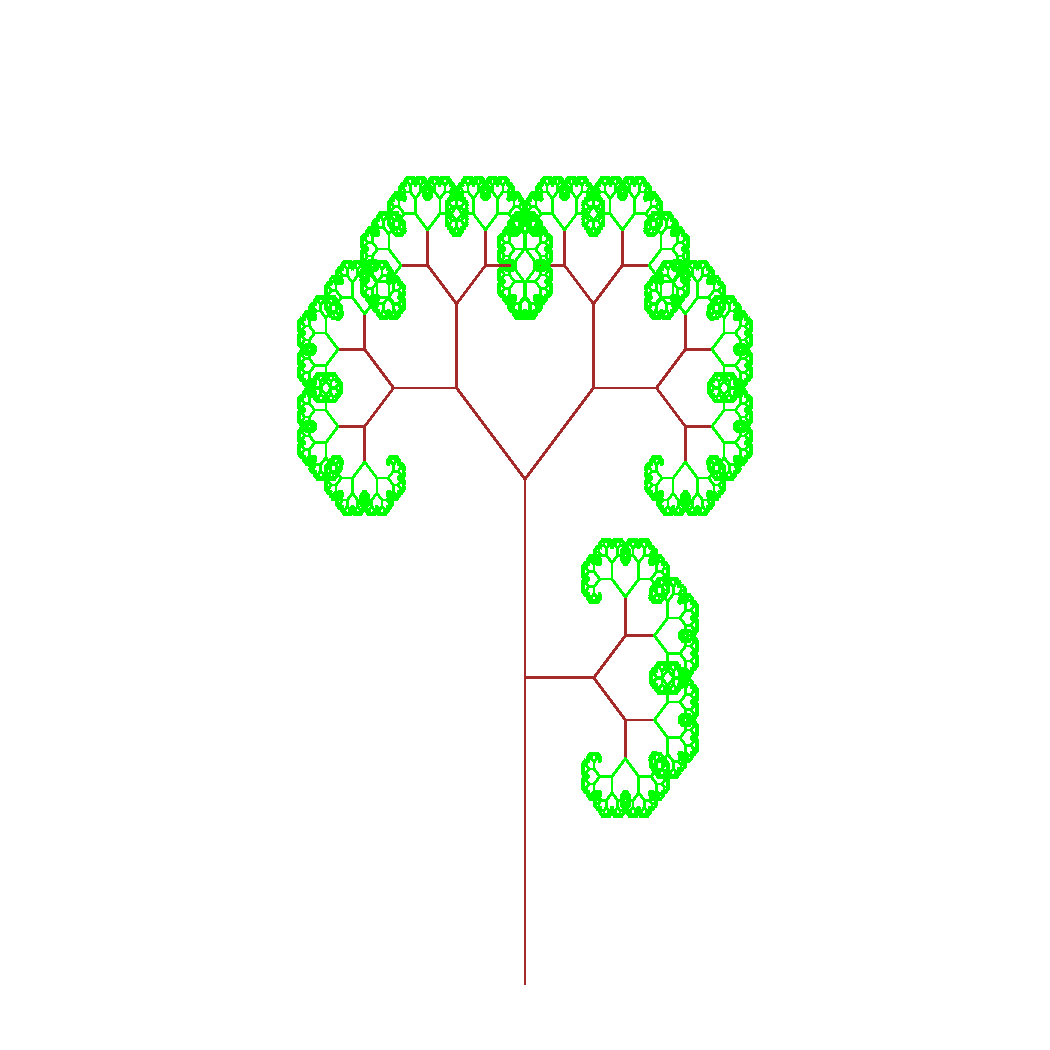
\includegraphics[width=0.5\linewidth]{../Results/Challenge_F_Tree.pdf}
\end{figure}

\end{document}